\customchapter[January 16, 2023]{Lecture 5: Non Deterministic Fnite Automata}

Continuing \href{Example 4.4}{Example 4.4}

\begin{figure}[!h]
    \centering
    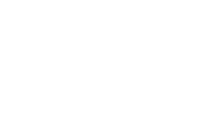
\includegraphics[width=0.5\textwidth]{figures/default.png}
    \caption{Solution to the above example}
\end{figure}

Define $L^2 = \{ ; w_1, w_2 \in \{a, b\}^{+} \}$

\begin{figure}[!h]
    \centering
    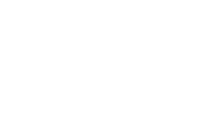
\includegraphics[width=0.5\textwidth]{figures/default.png}
    \caption{Solution to the $L^2$ example}
\end{figure}

\section{Non Deterministic Fnite Automata (NFA)}

% Ref DFA to its defination 
Inconvinences in DFA : 

\begin{itemize}
    \item We needed to introduce all the states wheather or not they serve any meaningful purpose. 
    \item in DFA, transition function is a complete function. 
    \item We can't leave arrows hanging. 
\end{itemize}

% fix sigma to E in DFA notes

\begin{definition}{NFA}
    An NFA is defined by $\bbM = ( \bbQ, \Sigma, \bbD, \bbQ_0, \bbF )$ where $\bbQ, \Sigma, \bbQ_0, \bbF$ are same as in DFA, but $$
    \bbD : \bbQ * (\Sigma \cap \{\ \lm \} ) \rightarrow 2^{Q} \text{ Power set of Q}$$
\end{definition}

\begin{example}
    $\bbD (q_1, a) = \{q_2, q_3\} $ and $\bbD(q_i, \lm) = \{q_i, q_j\} $
\end{example}

\begin{itemize}
    \item can have empty strings now
    \item machine can move from one state to another without processing any input
    \item any state with a path label $w$ can end up in a subset of final states 
\end{itemize}

\section{NFA Acceptance}

\begin{example}
    Consider the following NFA
\end{example}

\begin{figure}[!h]
    \centering
    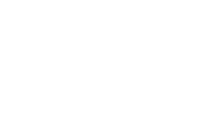
\includegraphics[width=0.5\textwidth]{figures/default.png}
    \caption{Solution to the above example}
\end{figure}

\begin{definition}{NFA Acceptance}
    The Language accepted by NFA $M$ is $L(M) = \{w \in \Sigma^{*}, \bbD^{*}(q_0, w) \int  F \neq \phi \} $
\end{definition}

\textbf{\underline{Remark}} It may end up in a non-final state but it must have atleast one element from final state. \\ 

Lanuguage accepted by Example 5.2 is $L(M) = \{a^3\} \cap \{a^{2n} : n \geq 1\} $

\begin{definition}{Extended Transition function}
    $\bbD^{*} is defined \bbD^{*}(q_i, w)$ contains $q_j$ iff there is a walk from $q_i$ to $q_j$ laveled $w$ in transition graph. 
\end{definition}

\begin{example}
    Consider this NFA
\end{example}

\begin{figure}[!h]
    \centering
    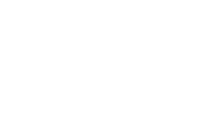
\includegraphics[width=0.5\textwidth]{figures/default.png}
    \caption{Solution to the above example}
\end{figure}

$L(M) = \{ (10)^n : n \geq 0\} $

\begin{definition}{Dead Configuration}
    A state from which you can't go anywhere. It has no outgoing arrow
\end{definition}

\begin{definition}{Equivalent Automata}
    If two automation accept the same language. $$
    M_1 \approx M_2 \text{ if } L(M_1) = L(M_2) $$ 
\end{definition}

\section{Convert from DFA to NFA}

$\oint$ Find a DFA that accepts $L(M_2)$ ?

\begin{figure}
    \centering
    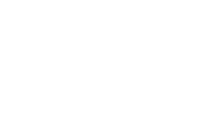
\includegraphics[width=0.5\textwidth]{figures/default.png}
    \caption{Solution to the above example}
\end{figure}




